% Cuadros originales compartidos por Oliver el 2 de septiembre de 2026.
% Mismo contenido incorporado a FPC; solo se recortan márgenes vacíos.

\begin{frame}{Plan financiero de julio: proyecciones 2026 y 2027}
  \centering
  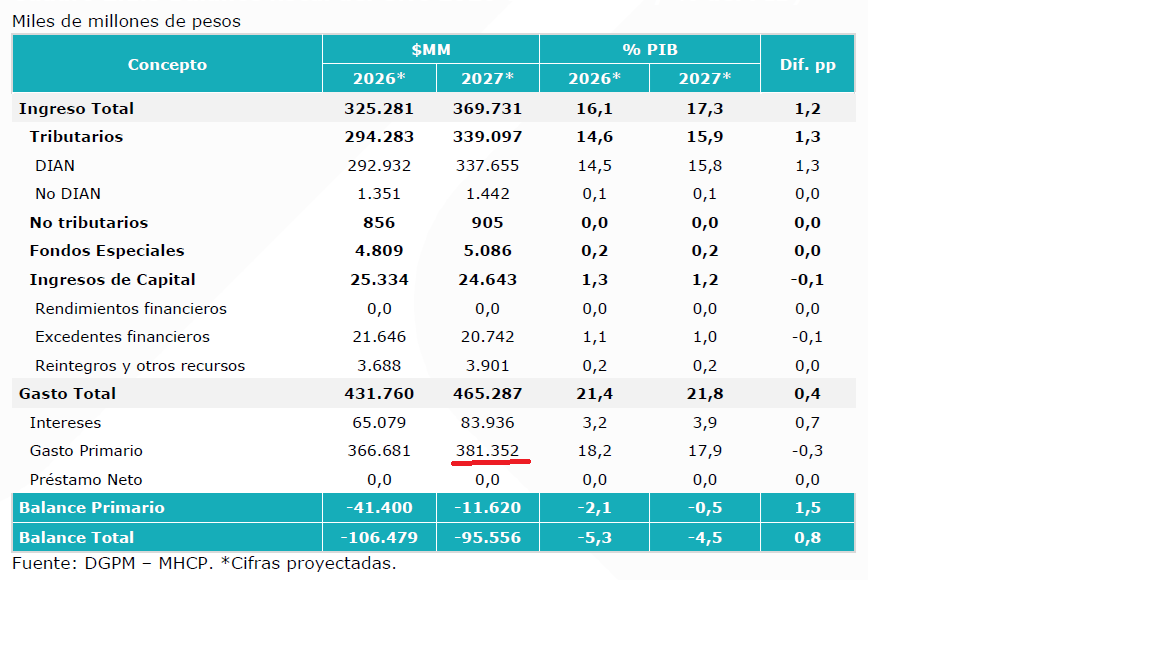
\includegraphics[
    width=\textwidth,
    height=0.83\textheight,
    keepaspectratio,
    trim=0bp 48bp 213bp 0bp,
    clip
  ]{assets/balance_fiscal_pf_julio_2027.png}
  \note{[Sources] DGPM -- Ministerio de Hacienda y Crédito Público. Cuadro del Plan Financiero de julio de 2026 con proyecciones para 2026 y 2027, reproducido en FPC, slides/BalanceFiscalPGN2027.tex. Imagen proporcionada por Oliver Pardo: HQ1MN6rW4AAZYve.png. Se conservan las cifras, la fuente y la indicación de proyecciones del original.}
\end{frame}

\begin{frame}{Balance fiscal 2027: MFMP, PGN y actualización}
  \centering
  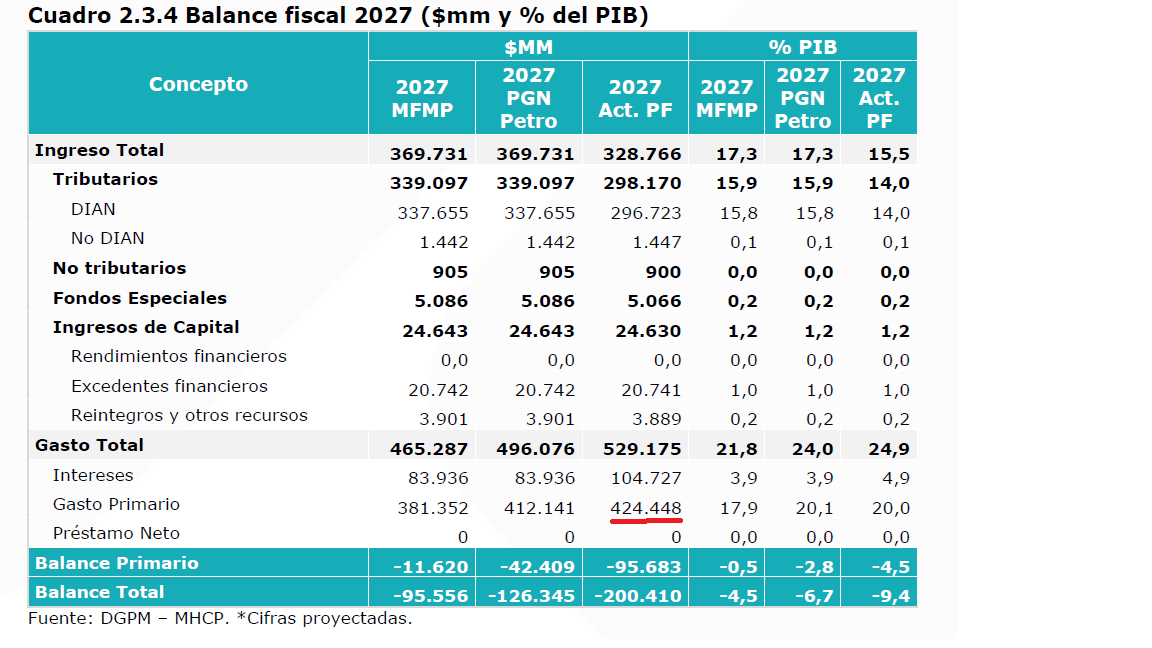
\includegraphics[
    width=\textwidth,
    height=0.77\textheight,
    keepaspectratio,
    trim=9bp 7.5bp 144bp 0bp,
    clip
  ]{assets/balance_fiscal_pgn2027_actualizado.png}

  \vspace{0.05cm}
  \parbox{0.94\textwidth}{\centering\scriptsize
    Nota: se reproduce el cuadro original. Los porcentajes de gasto y balances de ``PGN Petro'' no son consistentes con sus cifras en pesos.
  }
  \note{[Sources] DGPM -- Ministerio de Hacienda y Crédito Público. Anexo al Mensaje Presidencial del proyecto reformulado de PGN 2027, cuadro 2.3.4, página impresa 193; reproducido en FPC, slides/BalanceFiscalPGN2027.tex. Imagen proporcionada por Oliver Pardo: HQ1M7KqWYAA6u51.png. Se conservan las cifras publicadas y la indicación de proyecciones. No se corrigen los porcentajes de la columna ``PGN Petro''; se mantiene la advertencia de FPC sobre su inconsistencia con los montos nominales.}
\end{frame}
